\documentclass[10pt,letterpaper]{article}
\usepackage[lmargin=2.2in,rmargin=0.7in,
            tmargin=1.0in,bmargin=1.0in]{geometry}
\usepackage{notes}

\begin{document}

\begin{center}
\Large\textbf{3.6 - Impulsive Forces}\\
\normalsize (Section 3.4)
\end{center}

%%%%%%%%%%%%%%%%%%%%%%%%%%%%%%%%%%%%%%%%%%%%%%%%%%%%%%%%%%%%%%%%%%%%%%%%
\section{The Dirac Delta Function}

\subsection{Motivation}
In a forced spring equation, the right-hand side represents
an external force. We can use the Heaviside function to
switch a force on or off at time $t=a$:
\[
ax''+bx'+cx=
\underbrace{f(t)H(t-a)}_{\text{turn on at }t=a},
\quad \text{or}\quad
ax''+bx'+cx=
\underbrace{f(t)\bigl[1-H(t-a)\bigr]}_{\text{turn off at }t=a}.
\]
What if an effect lasts only for a very short time?
For example, striking a mass with a hammer, a brief burst of light, rapidly injecting a drug into the bloodstream. We idealize these brief events as
\textbf{instantaneous impulses}. To represent them,
we use the Dirac delta function $\delta(t)$:
\[
ax''+bx'+cx=
\underbrace{\delta(t-a)}_{\text{impulse at }t=a}.
\]

\subsection{Definition of $\delta(t)$}
The Dirac delta function $\delta(t)$ is defined in terms of rectangular pulses. Consider the parameterized rectangular function
\[
d_\tau(t)=
\begin{dcases}
\dfrac{1}{2\tau}, & -\tau<t<\tau,\\
0, & \text{otherwise},
\end{dcases}
\qquad \text{where }\tau>0.
\]
When $d_\tau(t)$ is sketched, it appears as a rectangle with a width of $2\tau$ and a height of $1/(2\tau)$, so its area is always one. That means the integral of $d_\tau$ is one as well:
\[\text{Area}=\text{width}\times\text{height}=
\int_{-\infty}^{\infty}d_\tau(t)\,dt
=1.
\]
This is true for any value of $\tau$.
As $\tau\to0^+$, the pulse becomes narrower and taller
while retaining the same area. This approximates an
impulse at $t=0$. The \textbf{Dirac delta} function $\delta(t)$ is defined to be 
$$
    \delta(t)=\lim_{\tau\to 0^+} d_{\tau}(t).
$$

\begin{figure}[H]
\centering
\begin{subfigure}[t]{0.46\linewidth}
\centering
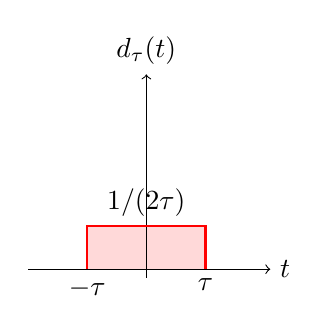
\begin{tikzpicture}[x=0.75cm,y=0.55cm]
    \fill[red!15] (-1,0) rectangle (1,1);

    \draw[->] (-2,0) -- (2.1,0) node[right] {$t$};
    \draw[->] (0,-0.2) -- (0,4.5)
        node[above] {$d_\tau(t)$};

    \draw[red,thick] (-1,0) -- (-1,1)
        -- (1,1) -- (1,0);

    \node[below] at (-1,0) {$-\tau$};
    \node[below] at (1,0) {$\tau$};
    \node[above] at (0,1) {$1/(2\tau)$};

\end{tikzpicture}
\caption{A rectangular pulse of area $1$.}
\end{subfigure}
\begin{subfigure}[t]{0.50\linewidth}
\centering
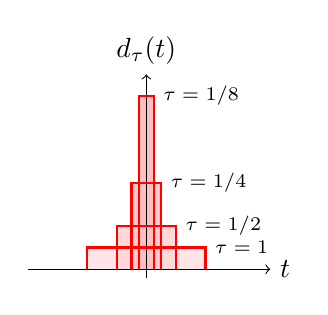
\begin{tikzpicture}[x=0.75cm,y=0.55cm]
    \fill[red!10] (-1,0) rectangle (1,0.5);
    \fill[red!15] (-0.5,0) rectangle (0.5,1);
    \fill[red!20] (-0.25,0) rectangle (0.25,2);
    \fill[red!25] (-0.125,0) rectangle (0.125,4);

    \draw[->] (-2,0) -- (2.1,0) node[right] {$t$};
    \draw[->] (0,-0.2) -- (0,4.5)
        node[above] {$d_\tau(t)$};

    \foreach \w/\h in {1/0.5,0.5/1,0.25/2,0.125/4}{
        \draw[red,thick] (-\w,0) -- (-\w,\h)
            -- (\w,\h) -- (\w,0);
    }

    \node[right] at (1,0.5) {\scriptsize $\tau=1$};
    \node[right] at (0.5,1) {\scriptsize $\tau=1/2$};
    \node[right] at (0.25,2) {\scriptsize $\tau=1/4$};
    \node[right] at (0.125,4) {\scriptsize $\tau=1/8$};
\end{tikzpicture}
\caption{Narrower pulses have greater height.}
\end{subfigure}
\caption{The delta is an idealized limit of pulses with
fixed area. This limit is understood through integration,
rather than as an ordinary pointwise limit.}
\end{figure}


The delta function models an instantaneous impulse.
Because its total area is $1$, we call it a
\textbf{unit impulse}. We can adjust its strength
and timing:
\[
f(t)=J\,\delta(t-a).
\]
This represents an impulse of strength $J$ applied
at time $t=a$. In a spring-mass model, $J$ is measured
in newton-seconds (N$\cdot$s). Its sign determines
the direction of the impulse.
\subsection{The Sifting Property}

\begin{theorem}[Sifting Property]
For a function $f$ continuous at $t=a$,
\[
\boxed{
\int_{-\infty}^{\infty}f(t)\delta(t-a)\,dt=f(a).
}
\]
\end{theorem}

The delta selects the value of $f$ at the impulse time.
If the integral is over a smaller interval, the same
rule applies when $a$ lies inside that interval.
If $a$ lies outside it, the integral is zero.

\begin{proof}
Assume $f$ is continuous near $a$ and approximate
$\delta(t-a)$ by $d_\tau(t-a)$. Then
\[
\int_{-\infty}^{\infty}f(t)d_\tau(t-a)\,dt
=\frac{1}{2\tau}\int_{a-\tau}^{a+\tau}f(t)\,dt.
\]
By the mean value theorem for integrals, this equals
$f(c_\tau)$ for some $c_\tau\in[a-\tau,a+\tau]$.
As $\tau\to0^+$, we have $c_\tau\to a$, so
\[
\lim_{\tau\to0^+}
\int_{-\infty}^{\infty}f(t)d_\tau(t-a)\,dt=f(a).
\]
This gives the sifting property.
\end{proof}

\begin{example}[1]{
Evaluate:
\[
\text{(a) }\int_{-\infty}^{\infty}
\cos t\,\delta(t-\pi)\,dt,
\qquad
\text{(b) }\int_{-\infty}^{\infty}
t^2\delta(t+3)\,dt,
\]
}

\paragraph{(a)}
The impulse occurs at $t=\pi$, so
\[
\int_{-\infty}^{\infty}\cos t\,\delta(t-\pi)\,dt
=\cos\pi=\boxed{-1}.
\]

\paragraph{(b)}
Write $\delta(t+3)=\delta(t-(-3))$.
The impulse occurs at $t=-3$:
\[
\int_{-\infty}^{\infty}t^2\delta(t+3)\,dt
=(-3)^2=\boxed{9}.
\]
\end{example}

%-------------------------------------------------------------
\subsection{Transform Formulas}

Here is the formula for the Laplace transform of the delta function
\[
\mathcal L[\delta(t)]=1.
\]
This is formula number 10 in the Laplace table of transforms. For $a>0$, we have shifted delta function
\[
\mathcal L[\delta(t-a)]
=\int_0^\infty e^{-st}\delta(t-a)\,dt
=e^{-as}.
\]
This is formula number 11. We can use this to solve models with impulsive forcing.

%%%%%%%%%%%%%%%%%%%%%%%%%%%%%%%%%%%%%%%%%%%%%%%%%%%%%%%%%%%%%%%%%%%%%%%%
% \section{First-Order IVPs}

% \subsection{Solving with an Impulse}

% The Laplace procedure is unchanged:
% \begin{enumerate}
%     \item Transform the DE and solve for $X(s)$.
%     \item Invert the rational parts.
%     \item Apply the switching property and write the
%     solution piecewise.
% \end{enumerate}
% Although the forcing contains a delta, the solution
% will contain a Heaviside function.

% \begin{example}[2]{
% Solve the IVP using Laplace transforms:
% \[
% x'=0.25x-2+5\delta(t-3),
% \qquad x(0)=6.
% \]
% Write the solution in Heaviside and piecewise forms.
% }

% \paragraph{Step 1. Transform and solve for $X(s)$.}
% Taking transforms gives
% \[
% sX(s)-6=0.25X(s)-\frac2s+5e^{-3s}.
% \]
% Therefore,
% \[
% X(s)=\frac{6}{s-0.25}
% -\frac{2}{s(s-0.25)}
% +5e^{-3s}\frac{1}{s-0.25}.
% \]

% \paragraph{Step 2. Invert the rational parts.}
% Partial fractions give
% \[
% \frac{1}{s(s-0.25)}
% =-\frac4s+\frac4{s-0.25}.
% \]
% Substituting and combining terms,
% \[
% X(s)=\frac8s-\frac2{s-0.25}
% +5e^{-3s}\frac{1}{s-0.25}.
% \]
% The unshifted part has inverse $8-2e^{0.25t}$.
% For the delayed term, the base inverse is
% \[
% g(t)=\mathcal L^{-1}
% \left[\frac{1}{s-0.25}\right]=e^{0.25t}.
% \]

% \paragraph{Step 3. Apply the delay.}
% Using the switching property,
% \[
% \boxed{
% x(t)=8-2e^{0.25t}
% +5H(t-3)e^{0.25(t-3)}.
% }
% \]
% In piecewise form,
% \[
% \boxed{
% x(t)=
% \begin{dcases}
% 8-2e^{0.25t}, & 0\le t<3,\\
% 8-2e^{0.25t}+5e^{0.25(t-3)}, & t\ge3.
% \end{dcases}
% }
% \]
% \end{example}

% %-------------------------------------------------------------
% \subsection{The Jump in the Solution}

% The one-sided limits at $t=3$ are
% \[
% x(3^-)=8-2e^{0.75},
% \qquad
% x(3^+)=8-2e^{0.75}+5.
% \]
% Thus,
% \[
% \boxed{x(3^+)-x(3^-)=5.}
% \]
% The impulse causes an instantaneous jump whose size
% equals the coefficient of $\delta(t-3)$.

% \subsection{Population Interpretation}

% Interpret $x$ as a population measured in thousands.
% Without the impulse,
% \[
% x'=0.25x-2
% \]
% describes growth with constant harvesting.
% Its equilibrium is $x^*=8$.

% The initial population $x(0)=6$ is below equilibrium,
% so it declines. At $t=3$, an additional $5$ thousand
% individuals are introduced instantaneously. This raises
% the population above equilibrium, after which it grows.

% \begin{figure}[H]
% \centering
% \begin{tikzpicture}[x=0.75cm,y=0.35cm]
%     \draw[->] (0,0) -- (8.7,0) node[right] {$t$};
%     \draw[->] (0,0) -- (0,11.7) node[above] {$x(t)$};

%     % Equilibrium
%     \draw[gray,dashed] (0,8) -- (8,8);
%     \node[right] at (8,8) {$x^*=8$};

%     % Before and after the impulse
%     \draw[red,thick,domain=0:3,samples=100]
%         plot (\x,{8-2*exp(0.25*\x)});
%     \draw[red,thick,domain=3:8,samples=150]
%         plot (\x,{
%             8-2*exp(0.25*\x)
%             +5*exp(0.25*(\x-3))
%         });

%     % Jump
%     \pgfmathsetmacro{\yLeft}{8-2*exp(0.75)}
%     \pgfmathsetmacro{\yRight}{\yLeft+5}
%     \draw[dotted] (3,\yLeft) -- (3,\yRight);
%     \draw[red,fill=white] (3,\yLeft) circle (2pt);
%     \fill[red] (3,\yRight) circle (2pt);
%     \node[right] at (3,{(\yLeft+\yRight)/2})
%         {\small jump $5$};

%     \fill[red] (0,6) circle (2pt);
%     \node[left] at (0,6) {$6$};
%     \node[below] at (3,0) {$3$};
% \end{tikzpicture}
% \caption{The impulse raises the population above
% the equilibrium level.}
% \end{figure}

%%%%%%%%%%%%%%%%%%%%%%%%%%%%%%%%%%%%%%%%%%%%%%%%%%%%%%%%%%%%%%%%%%%%%%%%
\section{Impulsive Forces}

\subsection{Underdamped Spring with an Impulse}

Consider the spring-mass system
\[
x''+2x'+5x=0,
\qquad x(0)=x'(0)=0.
\]
The characteristic roots are $\lambda=-1\pm2i$,
so the system is underdamped. With zero initial
displacement and velocity, its solution is $x(t)=0$:
the mass remains at rest.
Now suppose the mass is struck impulsively at $t=5$ in the positive direction.
We model the impact by adding $\delta(t-5)$ to the
right-hand side.


\begin{example}[2]{
Solve the IVP using Laplace transforms:
\[
x''+2x'+5x=\delta(t-5),
\qquad x(0)=x'(0)=0.
\]
Write the solution in Heaviside and piecewise forms.
}

\paragraph{Step 1. Transform and solve for $X(s)$.}
Using the zero initial conditions,
\[
(s^2+2s+5)X(s)=e^{-5s}.
\]
Complete the square to obtain
\[
X(s)=e^{-5s}
\underbrace{\frac{1}{(s+1)^2+4}}_{G(s)}.
\]

\paragraph{Step 2. Invert the rational part.}
The transform contains both an exponential shift
and a time delay:
\[
X(s)=
\underbrace{e^{-5s}}_{\text{time delay}}
\frac{1}{\underbrace{(s+1)^2}_{\text{exponential shift}}+4}.
\]
Set $e^{-5s}$ aside. Since
\[
\mathcal L^{-1}\left[\frac{1}{s^2+4}\right]
=\frac12\sin2t,
\]
the exponential shift gives
\[
g(t)=\mathcal L^{-1}[G(s)]
=\frac12e^{-t}\sin2t.
\]

\paragraph{Step 3. Apply the delay.}
Delay the entire function $g(t)$ by $5$:
\[
x(t)=H(t-5)g(t-5).
\]
Therefore,
\[
\boxed{
x(t)=\frac12H(t-5)e^{-(t-5)}
\sin\bigl(2(t-5)\bigr).
}
\]
In piecewise form,
\[
\boxed{
x(t)=
\begin{dcases}
0, & 0\le t<5,\\
\frac12e^{-(t-5)}\sin\bigl(2(t-5)\bigr),
& t\ge5.
\end{dcases}
}
\]
\end{example}

%-------------------------------------------------------------
\subsection{Position and Velocity at Impact}

We use the notations $x(a^+)$ and $x(a^-)$ to denote one sided limits from the right and left sides, respectively. These are useful for describing jumps. Adding the forcing term $\delta(t-5)$ creates a jump in the velocity $x'$, but not in the position $x$ at $t=5$:
\[
x(5^-)=x(5^+)=0,
\qquad
x'(5^-)=0,\quad x'(5^+)=1.
\]
This makes sense since the mass cannot magically teleport after being struck. More generally,
\[
mx''+\gamma x'+kx=J\delta(t-a)
\quad\implies\quad
x'(a^+)-x'(a^-)=\frac{J}{m}.
\]
A positive impulse increases the velocity; a negative impulse decreases it. This gives us a hint on how to plot the solution.

%-------------------------------------------------------------
\subsection{Sketching the Solution}

To sketch our solution:
\begin{enumerate}
    \item Before $t=5$, draw $x=0$.
    \item At $t=5$, keep the curve connected but
    change its slope from $0$ to $1$.
    \item After $t=5$, draw a decaying oscillation
    with period $\pi$.
\end{enumerate}

% Place the existing figure here.

\begin{figure}[H]
\centering
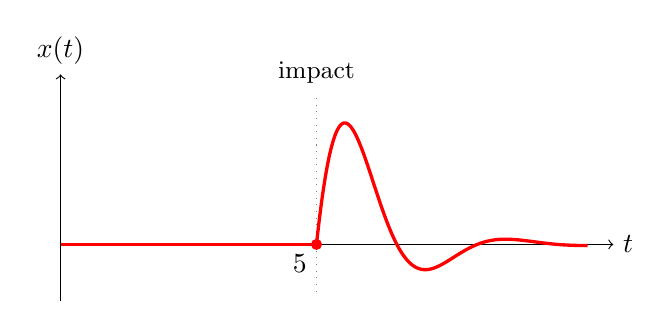
\begin{tikzpicture}[x=0.65cm,y=6cm]
    \draw[->] (0,0) -- (10.8,0) node[right] {$t$};
    \draw[->] (0,-0.12) -- (0,0.36)
        node[above] {$x(t)$};

    % Impact time
    \draw[dotted,gray] (5,-0.1) -- (5,0.32);
    \node[above] at (5,0.32) {\small impact};

    % Solution
    \draw[red,very thick] (0,0) -- (5,0);
    \draw[red,very thick,domain=5:10.3,samples=350]
        plot (\x,{
            0.5*exp(-(\x-5))*sin(deg(2*(\x-5)))
        });

    \fill[red] (5,0) circle (2pt);
    \node[below left] at (5,0) {$5$};
\end{tikzpicture}
\caption{The mass begins oscillating after the impulse.
Position is continuous, but its slope jumps at $t=5$.}
\end{figure}

In general, a spring may receive multiple impulses:
\[
mx''+\gamma x'+kx
=J_1\delta(t-a_1)+J_2\delta(t-a_2).
\]
The solution has the form
\[
x(t)=h(t)
+J_1H(t-a_1)g(t-a_1)
+J_2H(t-a_2)g(t-a_2),
\]
where $h(t)$ describes the motion from the initial
conditions and $g(t)$ is the response to a unit impulse
applied at time zero. At each impact, the position stays continuous and
the velocity changes by $J_i/m$. Depending on its
direction relative to the motion, an impulse can
speed up, slow down, or reverse the mass. 
\end{document}